% vim:set softtabstop=2 shiftwidth=2:

Fig.~\ref{fig:dambreak} depicts the evolution of the adaptive mesh for a
dam-break test case ran on ALCF Theta using two-phase
incompressible PHASTA-chef with data streams~\cite{Rod13} .
The dense fluid (water) is initially held against the left wall (not pictured)
in a square column created by a fictitious constraint representing a dam.
The remainder of the domain (1.25 column heights high and five column heights wide)
is air.
When the constraint is removed, as if the dam broke, the dense fluid falls and
advances to the right~\cite{Rod13}.
A distance and curvature-based refinement band tracks the air-water interface.
Outside of these bands the mesh is graded to a reference coarse size.

Algorithm~\ref{alg:twophase} lists the steps in the two-phase adaptive analysis.
Note, the terms `read' and `write' are used to describe transfers from and to
both streams and files.
On Lines~\ref{step:loadmesh}-\ref{step:loadprobdef} the
PUMI partitioned mesh, geometric model, and problem definition
information is loaded.
Next, the chef preprocessor is called on Line~\ref{step:preprocess}.
The preprocessor first executes adjacency-based mesh entity
reordering ($l.$\ref{step:reorder})~\cite{zhou2010adjacency}
to improve the efficiency of the assembly and linear algebra solution
procedures.
Next, it creates the finite element mesh (i.e.,
nodes and element connectivity), solution field, and structures containing the
point-to-point communication protocols and boundary conditions
($l.$\ref{step:preprocCreateMesh}-\ref{step:preprocCreateFields}).
Preprocessing concludes with the writing of this data to streams
($l.$\ref{step:preprocWrite}).

Line~\ref{step:loop} of Algorithm~\ref{alg:twophase} begins the solve-adapt
cycle that runs until the requested number of solver time steps is reached.
The PHASTA solver first reads its input information from chef via files or streams
($l$.\ref{step:loadChefFields}),
then executes an analyst-specified number of time steps ($l$.\ref{step:phastaSolve}),
and computes the distance-based mesh size field ($l$.\ref{step:computeSzField}).
The solver then sends the computed mesh size field and solution field to
files/streams.
Those fields are read on Line~\ref{step:attachPhastaFields} and attached to the
PUMI mesh.
Next, chef drives MeshAdapt with the mesh size
field ($l$.\ref{step:adapt}).
To prevent memory exhaustion during mesh refinement procedures, ParMETIS part
k-way graph re-partitioning (via Zoltan) is called using weights that
approximate the change in mesh element count on each part
($l$.\ref{step:predlb},~\ref{step:midlb}).
After adaptation, chef executes preprocessing as previously described
($l$.\ref{step:preprocessLoop}).

\begin{algorithm}
  \caption{Two-phase PHASTA-chef Adaptive Loop}\label{alg:twophase}
  \small
  \begin{algorithmic}[1]
    \Procedure{adaptiveLoop}{$max\_steps$}
      \State $pumi\_mesh \gets$ load the partitioned PUMI mesh
             from disk\label{step:loadmesh}
      \State $geom \gets$ load the geometric model from
             disk\label{step:loadgeom}
      \State $chef\_probdef \gets$ load the chef problem definition
             from disk\label{step:loadprobdef}
      \State \Call{preprocessor}{$pumi\_mesh$,$geom$,$chef\_probdef$}
             \label{step:preprocess}
      \State $step\_number \gets$ 0
      \While{$step\_number < max\_steps$\label{step:loop}}
        \State $step\_number \gets$ \Call{PHASTA}{$N$}
        \State \Call{readAndAttach}{$size\_field$,$phasta\_fields$,$pumi\_mesh$}
          \label{step:attachPhastaFields}
        \State \Call{meshadapt}{$pumi\_mesh$,$size\_field$,$max\_iterations$}
        \State \Call{ParMA}{vtx$>$elm,$pumi\_mesh$}\label{step:phastaParma}
        \State \Call{preprocessor}{$pumi\_mesh$,$geom$,$chef\_probdef$}
               \label{step:preprocessLoop}
      \EndWhile
    \EndProcedure

    \Procedure{preprocessor}
              {$pumi\_mesh$, $geom$, $chef\_probdef$}
      \State reorder the mesh entities holding
             degrees-of-freedom \label{step:reorder}
      \State $phasta\_mesh \gets$ create PHASTA mesh data
             structures \label{step:preprocCreateMesh}
      \State $phasta\_fields \gets$ create PHASTA field data
             structures \label{step:preprocCreateFields}
      \State write $phasta\_mesh$ and $phasta\_fields$ to
             files/streams \label{step:preprocWrite}
    \EndProcedure

    %SCOREC/core/ma/ma.cc
    \Procedure{PUMI meshadapt \label{step:adapt}}
              {$pumi\_mesh$,$size\_field$,$max\_iterations$}
      \State $w \gets$ per element field estimating
             the change in element volume based on $size\_field$
      \State predictively balance the mesh elements for
             element weight $w$ \label{step:predlb}
      \For{ $iteration \gets$ 0 \textbf{to} $max\_iterations$ }
         \State coarsen the mesh
         \State re-balance the mesh elements for element
                weight $w$ \label{step:midlb}
         \State refine the mesh
      \EndFor
      \State re-balance the mesh elements
    \EndProcedure

    \Procedure{PHASTA}{$N$}
      \State read $phasta\_mesh$, $phasta\_fields$ data from
      files/streams\label{step:loadChefFields}
      \State run the flow solver for $N$ steps\label{step:phastaSolve}
      \State $size\_field \gets$ isotropic size field based on distance to
      phasic interface\label{step:computeSzField}
      \State write the mesh $size\_field$ and $phasta\_fields$ to files/streams
    \EndProcedure
  \end{algorithmic}
\end{algorithm}

\begin{figure} \centering
    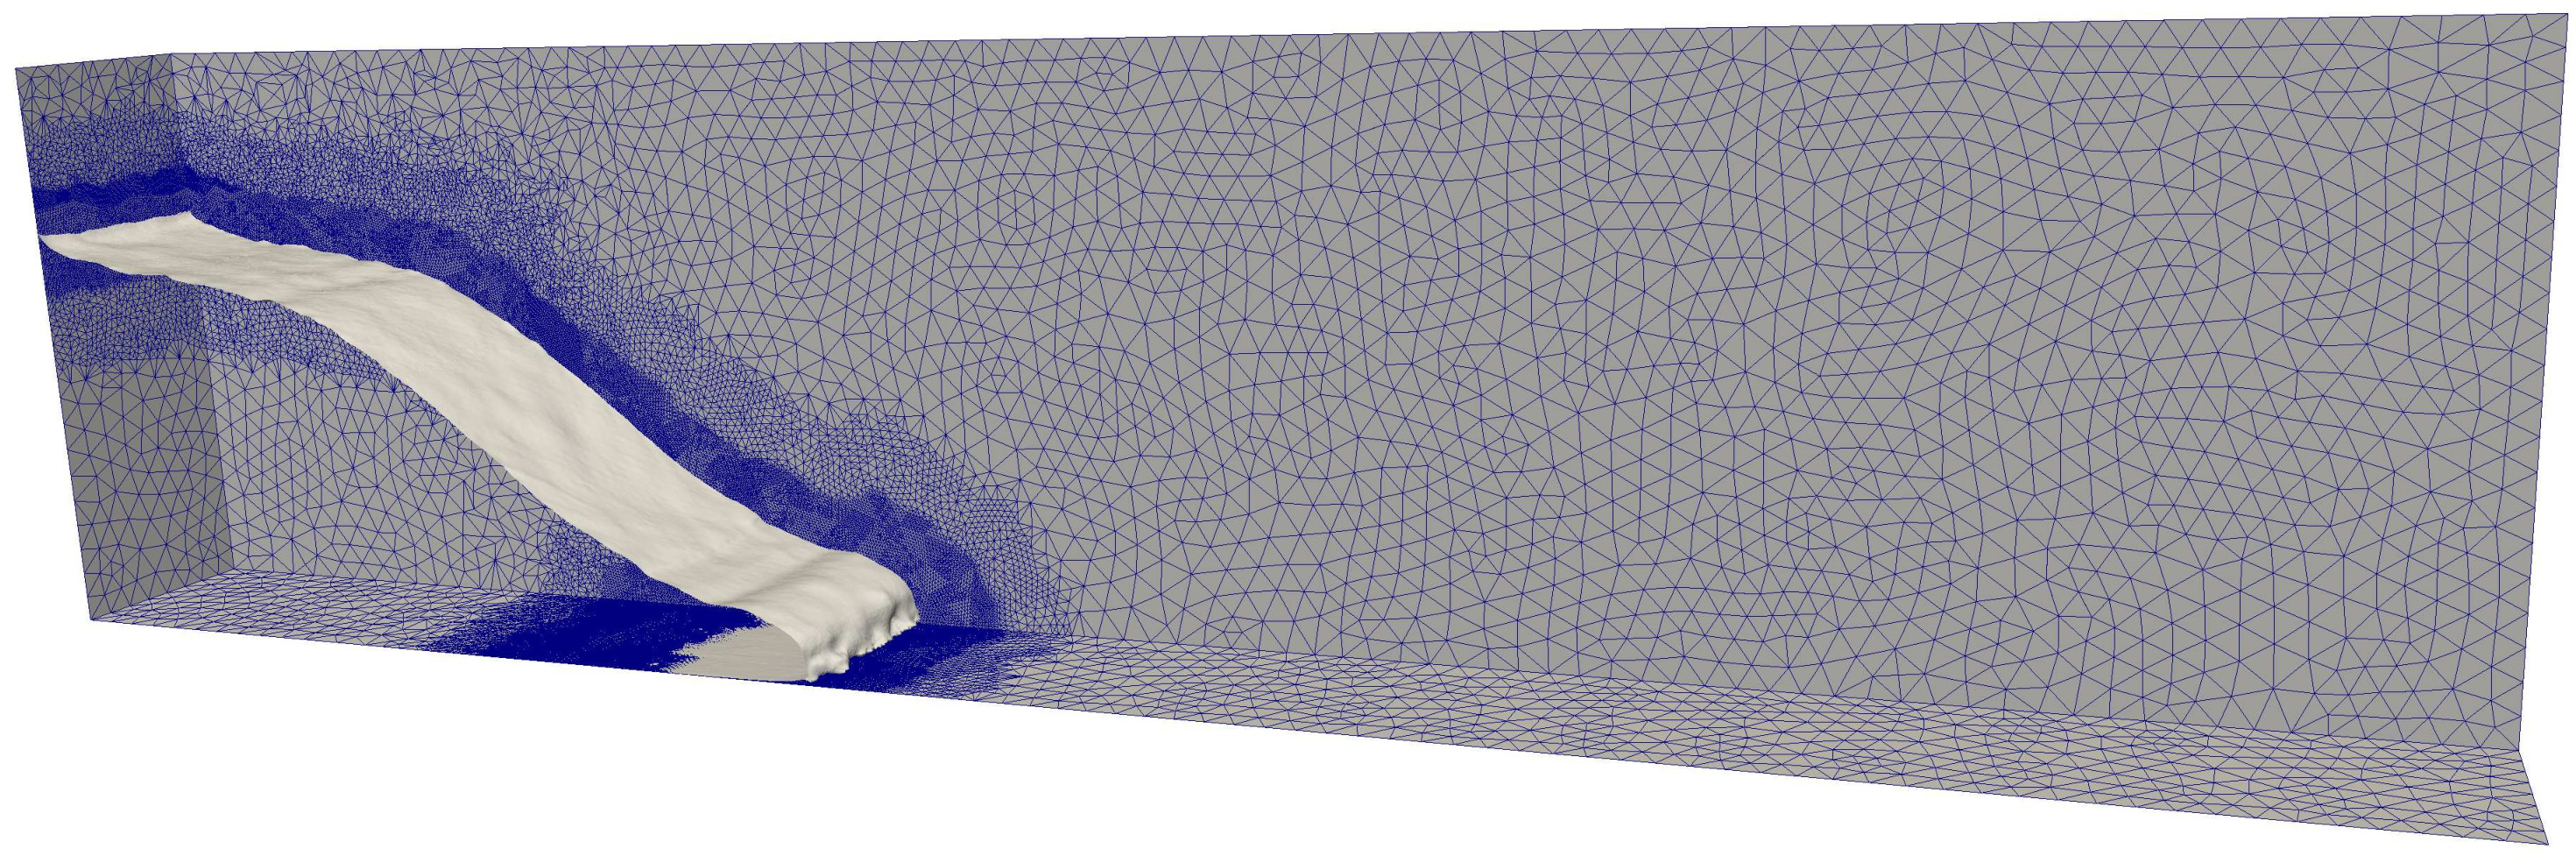
\includegraphics[width=.6\textwidth]{figures/dambreak/3DIso_420_cropped.jpg}
    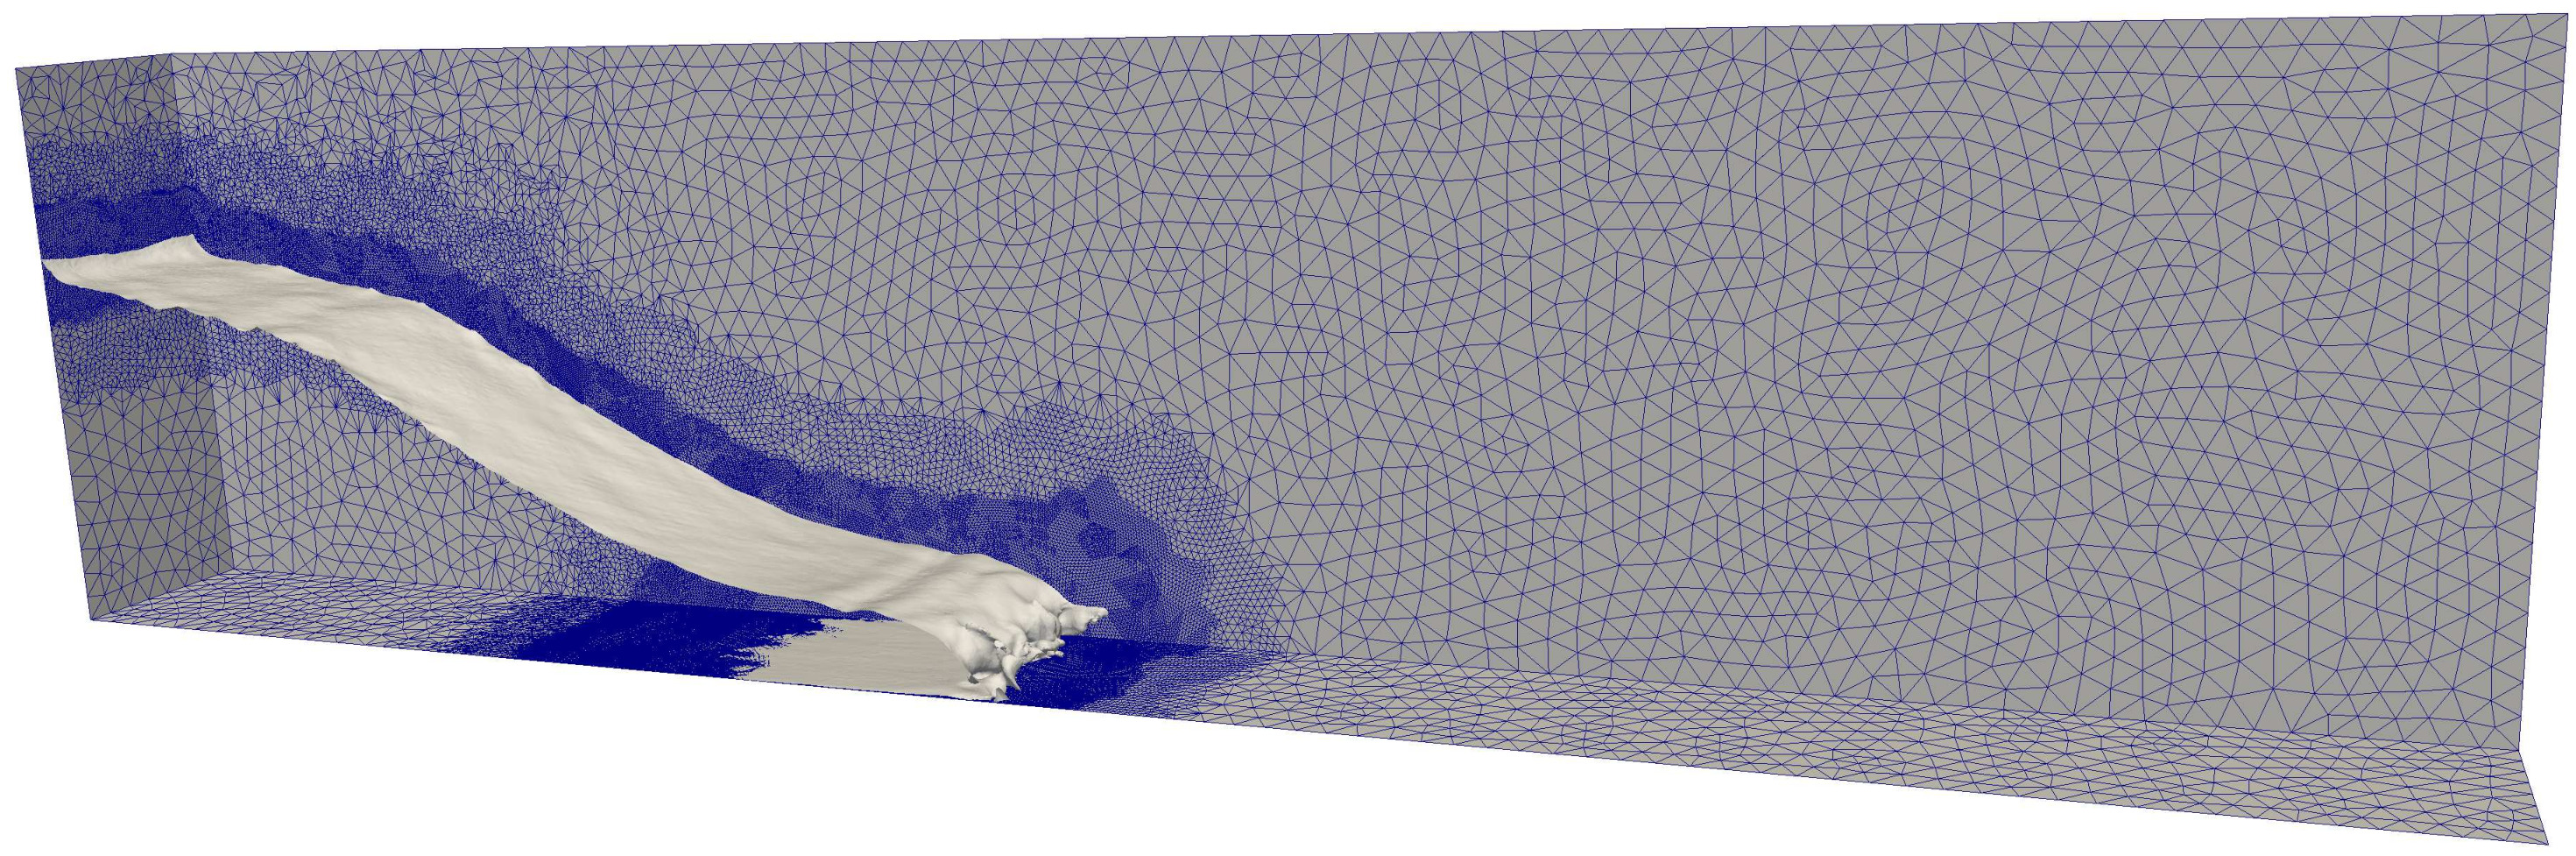
\includegraphics[width=.6\textwidth]{figures/dambreak/3DIso_520_cropped.jpg}
    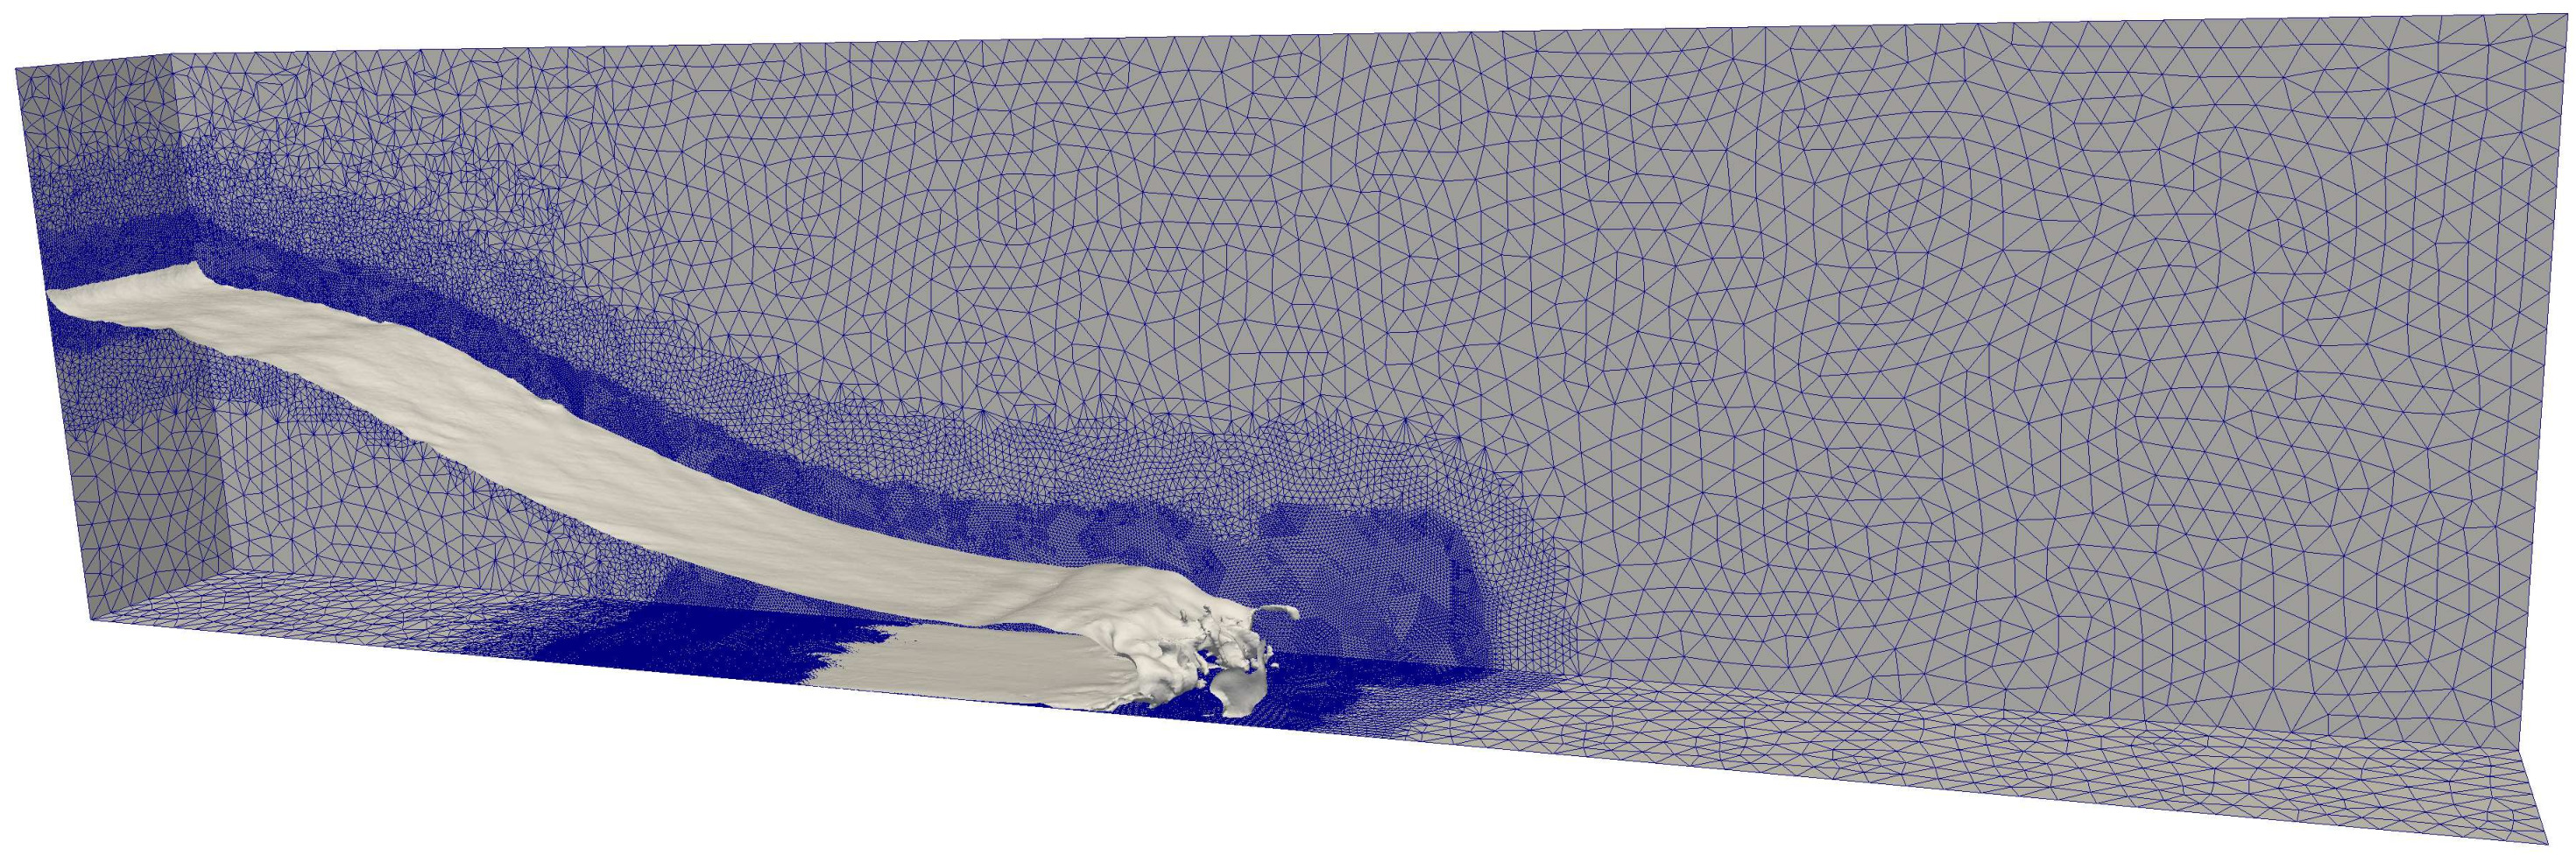
\includegraphics[width=.6\textwidth]{figures/dambreak/3DIso_620_cropped.jpg}
    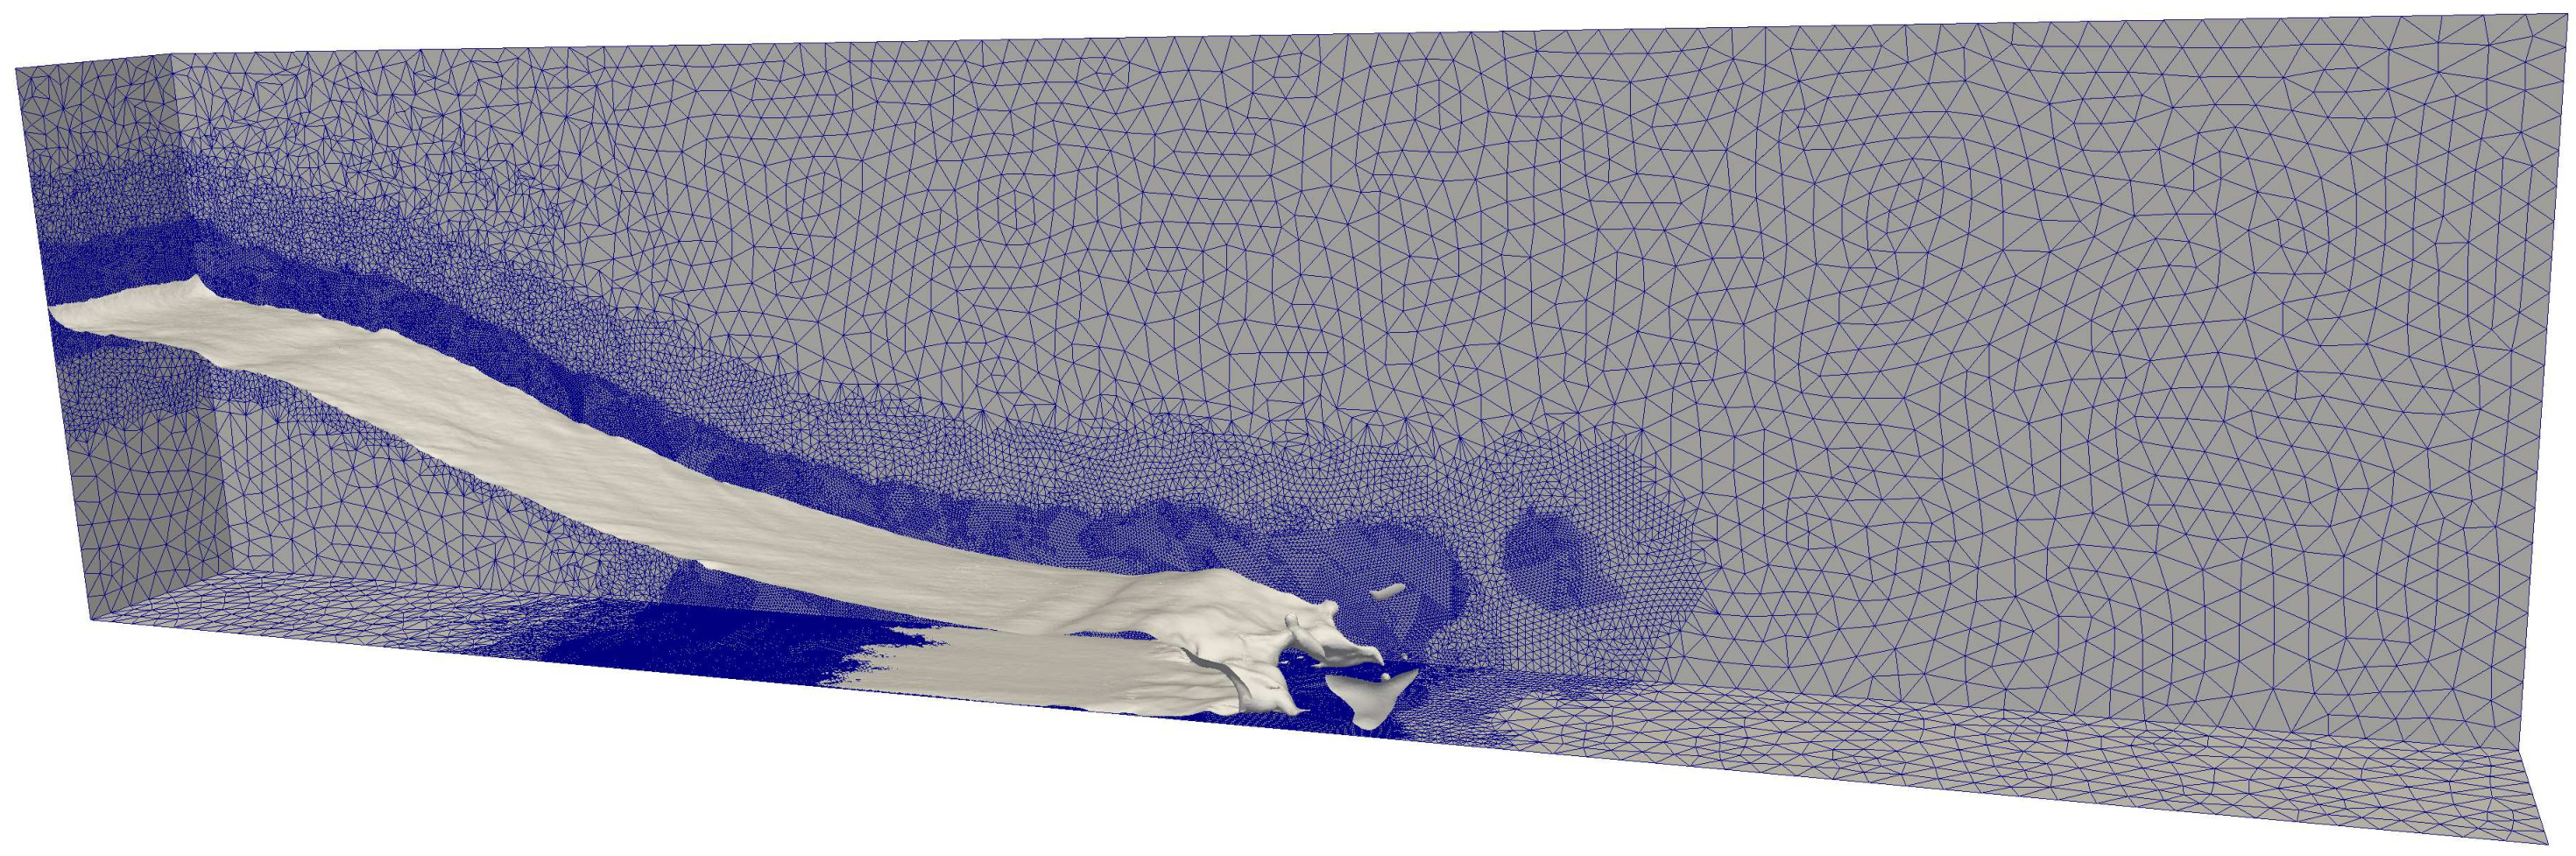
\includegraphics[width=.6\textwidth]{figures/dambreak/3DIso_720_cropped.jpg}
    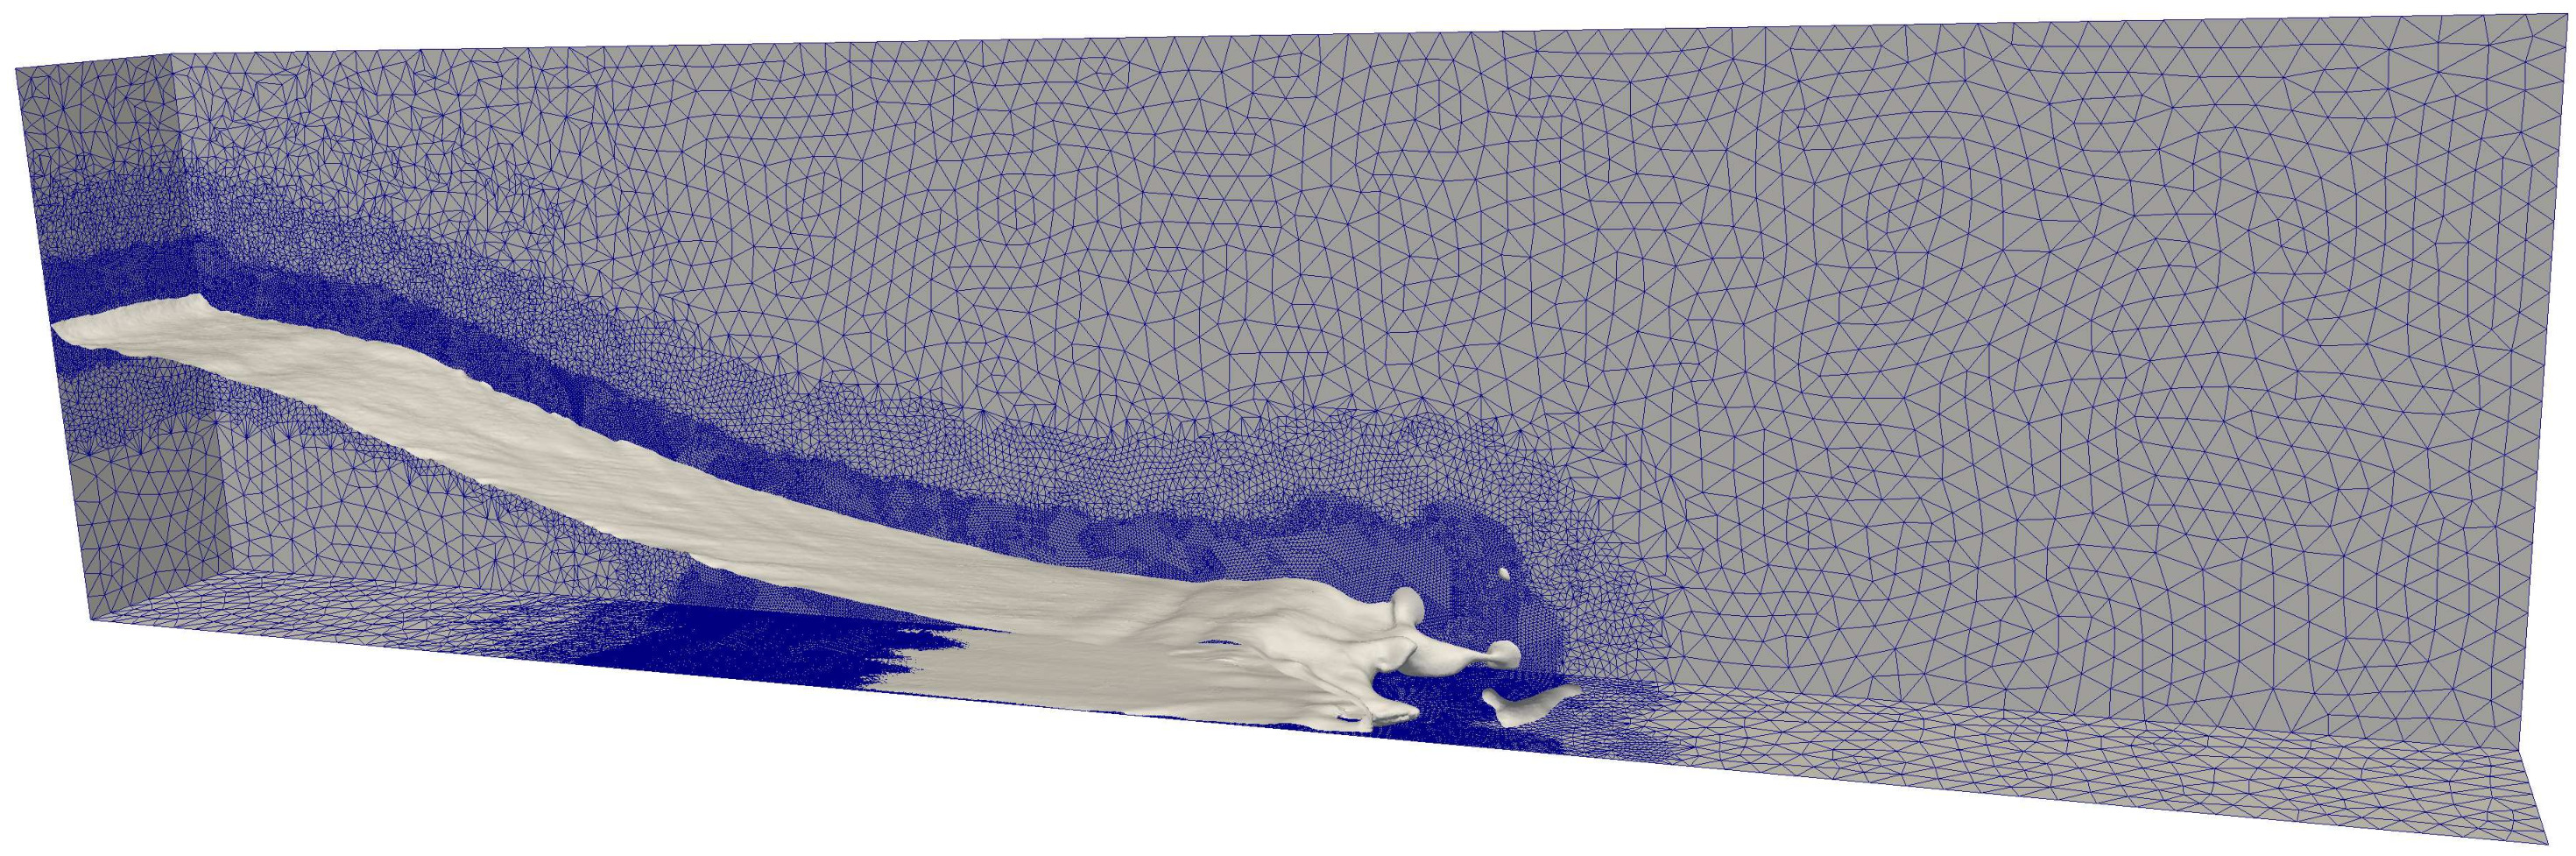
\includegraphics[width=.6\textwidth]{figures/dambreak/3DIso_820_cropped.jpg}
    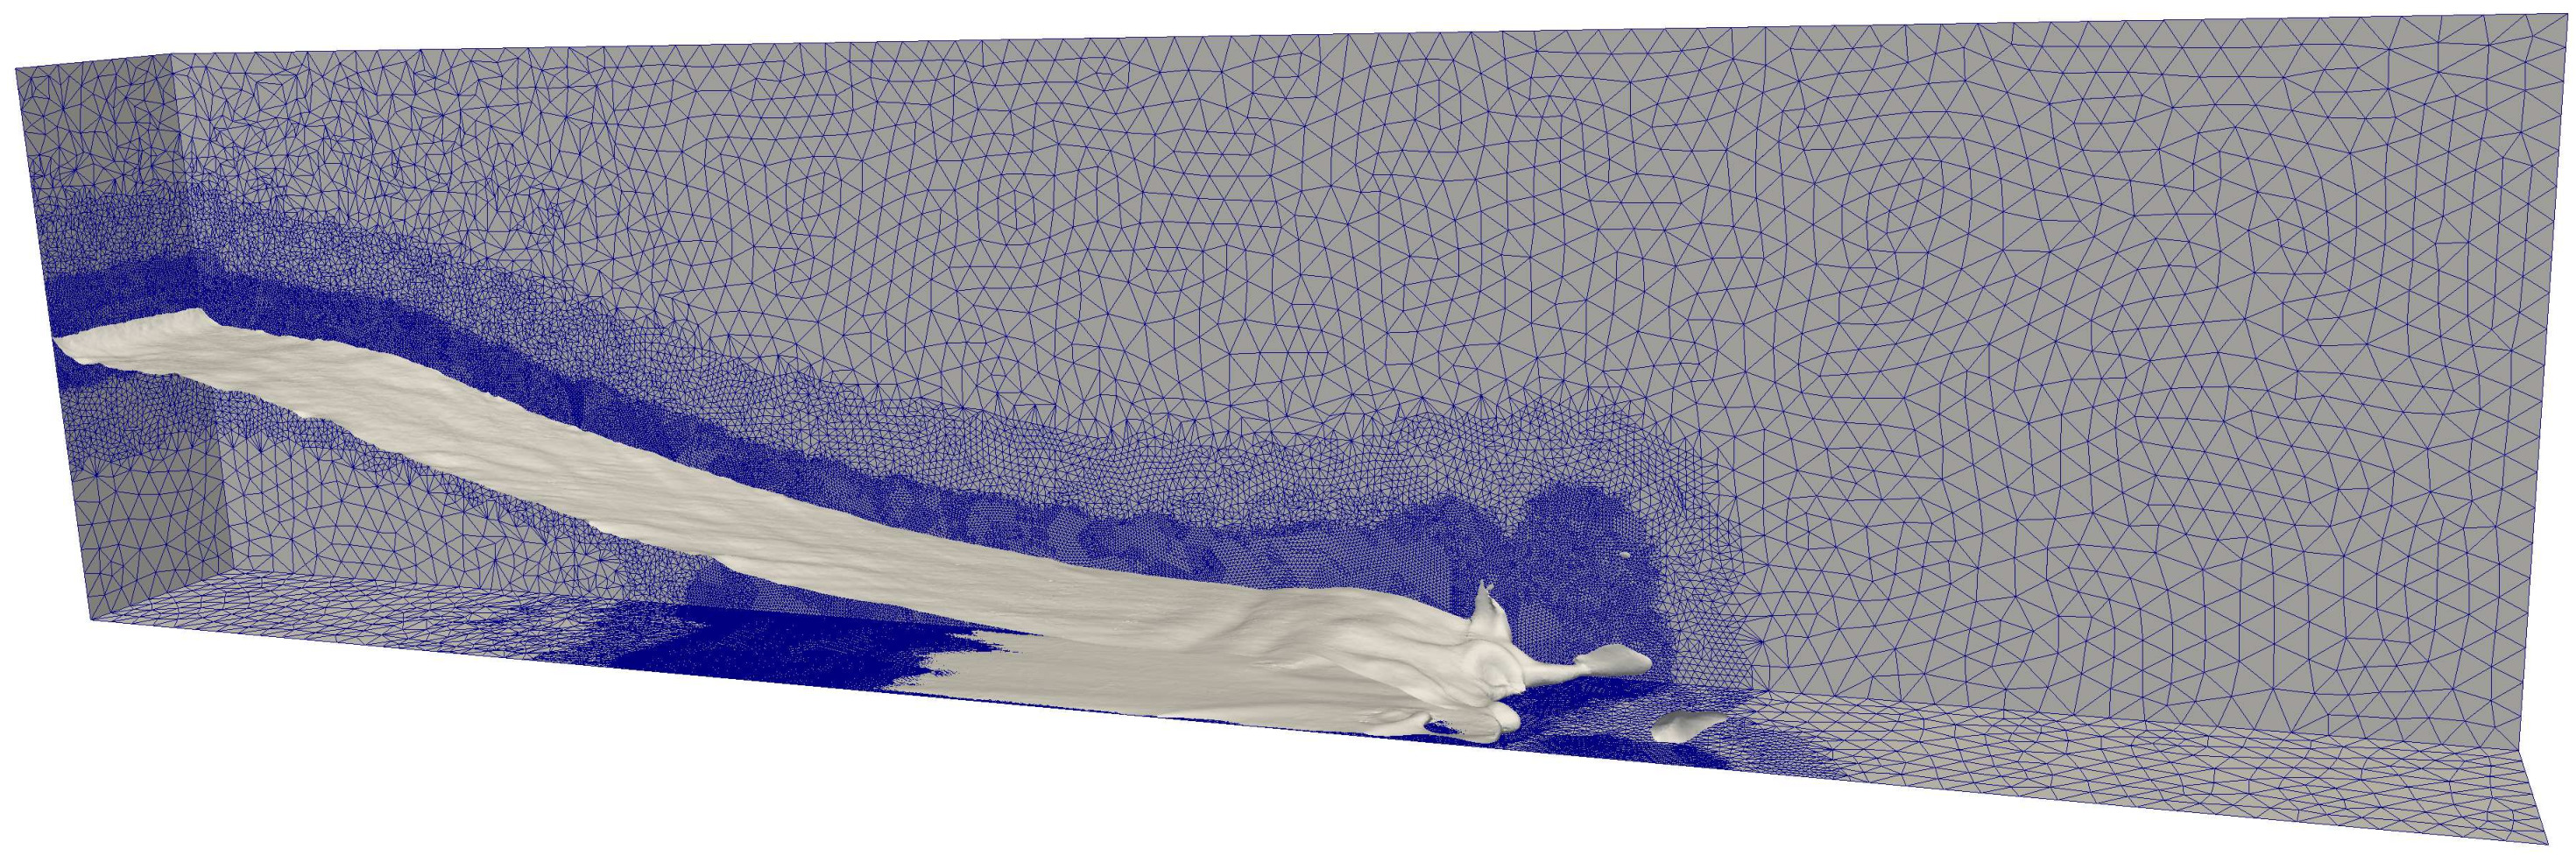
\includegraphics[width=.6\textwidth]{figures/dambreak/3DIso_920_cropped.jpg}
    \caption[Evolution of an adaptive dam-break case.]{
      Evolution of an adaptive dam-break case ran on 2048 processes of the ALCF
      Theta system using two-phase, incompressible PHASTA coupled to
      PUMI unstructured mesh adaptation with data streams.
      Each image (top to bottom) represents an advancement in
      physical time by 1/100 of a second.  %dt=0.0001 for theta job 63394
      The air-water phasic interface iso-surface is shown in gray.
    }
    \label{fig:dambreak}
\end{figure}
